\documentclass[11pt,letterpaper]{article}
\usepackage[margin=.65in,headheight=16pt,headsep=16pt,footskip=22pt]{geometry}
\usepackage[T1]{fontenc}\usepackage{helvet}\renewcommand{\familydefault}{\sfdefault}
\usepackage{tikz,fancyhdr}\pagestyle{fancy}\fancyhf{}
\fancyhead[L]{\small Week 56 / Corners of a solid / Preparation assets}
\fancyfoot[L]{\scriptsize Bellingham Math Circle / Week 56 / N56-M-v1}
\fancyfoot[R]{\scriptsize\thepage}
\renewcommand{\headrulewidth}{.35pt}\renewcommand{\footrulewidth}{.25pt}
\setlength{\parindent}{0pt}\setlength{\parskip}{7pt}
\newcommand{\net}[2]{\par\vspace{.15cm}\textbf{#1}\par\begin{center}\input{#2}\end{center}}
\begin{document}
Print at actual size, 100\%. Every face edge is 30 mm. Cut solid outside lines; fold dashed lines. Shaded tabs lie outside the faces. Join the two copies of each letter, with the shaded tab inside. Small blue corner numbers must meet matching numbers. Large numbers identify faces. Close every face.
\begin{center}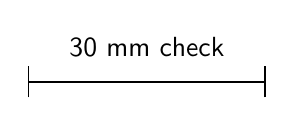
\begin{tikzpicture}[x=1mm,y=1mm]
\draw[line width=.8pt] (0,0)--(30,0);\draw (0,-2)--(0,2) (30,-2)--(30,2);
\node[above] at (15,2) {30 mm check};\end{tikzpicture}\end{center}
\net{Cube: six square faces}{cube-net.tex}
\vspace{.1cm}\net{Tetrahedron: four equilateral triangle faces}{tetrahedron-net.tex}
\newpage
Every face edge is 30 mm. Cut solid outside lines, fold dashed lines, join matching letters and blue corner numbers. Tabs do not count as faces.
\net{Octahedron: eight equilateral triangle faces}{octahedron-net.tex}
\vspace{.35cm}\net{Right triangular prism: two equilateral triangles and three squares}{triangular-prism-net.tex}
\newpage
Every face edge is 30 mm. Cut solid outside lines, fold dashed lines, join matching letters and blue corner numbers. Tabs do not count as faces.
\net{Square pyramid: one square and four equilateral triangles}{square-pyramid-net.tex}
\textbf{Equilateral triangle faces for corner fans}\par
Cut eight triangles. The black dot marks the corner to put at the center of a fan. Tape adjacent sides together; preserve each face's shape. These have no glue tabs.
\begin{center}
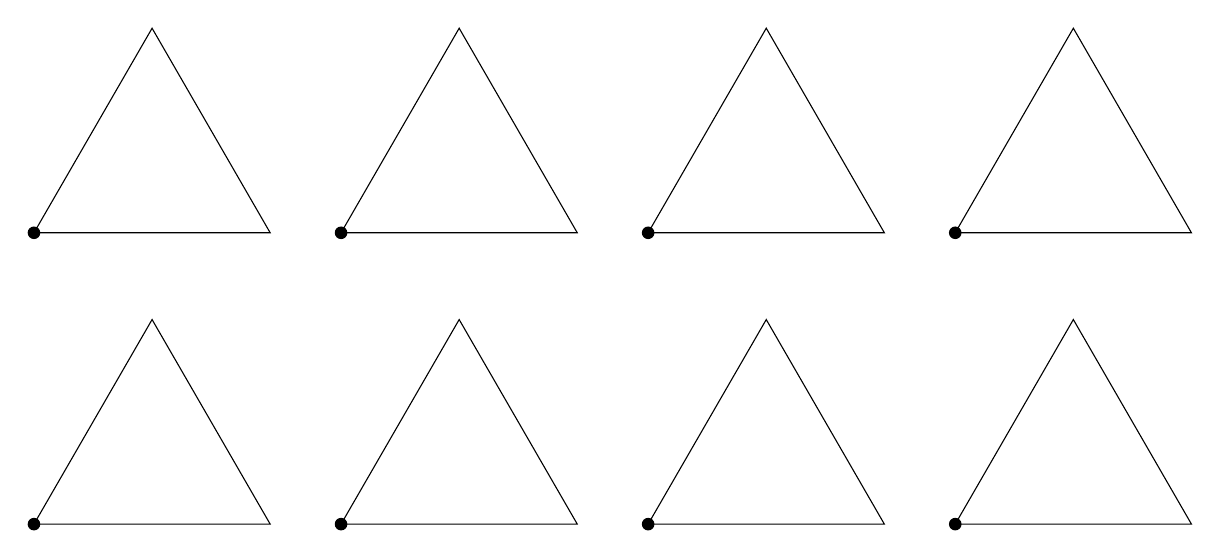
\begin{tikzpicture}[x=1mm,y=1mm,font=\sffamily\small]
\foreach \x in {0,39,78,117}{\foreach \y in {0,37}{
 \draw (\x,\y)--++(30,0)--++(-15,25.980762)--cycle;
 \fill (\x,\y) circle (.8mm);
}}
\end{tikzpicture}
\end{center}
\newpage
\textbf{Square faces for corner fans}\par
Cut eight squares. Every edge is 30 mm. The black dot marks the corner to put at the center of a fan. These have no glue tabs.
\begin{center}
\begin{tikzpicture}[x=1mm,y=1mm]
\foreach \x in {0,39,78,117}{\foreach \y in {0,41}{
 \draw (\x,\y) rectangle ++(30,30);\fill (\x,\y) circle (.8mm);
}}
\end{tikzpicture}
\end{center}
\vspace{1cm}
\textbf{Full-turn circles}\par
Cut two circles, each 80 mm across. Lay fan corners around the center dot to see the missing part of a turn.
\begin{center}
\begin{tikzpicture}[x=1mm,y=1mm]
\draw (0,0) circle (40);\fill (0,0) circle (.8mm);
\draw (90,0) circle (40);\fill (90,0) circle (.8mm);
\end{tikzpicture}
\end{center}
\end{document}
